% =====================================================================
%  What Does Formal Structure in Counterexample Feedback Buy?
%  NeurIPS 2026 Workshop on AI for Verifiable Coding
%
%  BUILD:  pdflatex main && bibtex main && pdflatex main && pdflatex main
%
%  Submission form: no options on the style package. That is the
%  ANONYMOUS version with line numbers, which is what the call requires.
%  Add [preprint] for arXiv, [final] only if accepted.
% =====================================================================

\documentclass{article}
\usepackage{neurips_2026_vericode}

\usepackage[T1]{fontenc}
\usepackage[utf8]{inputenc}
\usepackage{microtype}
\usepackage{amsmath,amssymb}
\usepackage{booktabs}
\usepackage{graphicx}
\usepackage{xcolor}
\usepackage{listings}
\usepackage[hidelinks]{hyperref}
\usepackage{url}

\definecolor{codegray}{gray}{0.45}
\lstdefinestyle{bt}{
  basicstyle=\ttfamily\scriptsize,
  commentstyle=\color{codegray}\itshape,
  morecomment=[l]{\#},
  showstringspaces=false,
  columns=fullflexible,
  breaklines=true,
  frame=single,
  framesep=3pt,
  rulecolor=\color{codegray},
  xleftmargin=0pt,
  aboveskip=4pt, belowskip=4pt,
}
\lstset{style=bt}

\newcommand{\rhoc}[1]{\rho_{#1}}
\newcommand{\Hnc}{H(\mathrm{node}\mid\mathrm{contract})}

\title{What Does Formal Structure in Counterexample Feedback Buy?}

\author{Anonymous Author(s)\\Affiliation\\Address\\\texttt{email}}

\begin{document}
\maketitle

\begin{abstract}
Counterexample-guided repair asks a synthesizer to fix a program given a
description of how it failed. When that synthesizer is a large language model,
the description can range from a raw execution trace to a formal certificate
carrying a violated predicate, a signed robustness value, a minimized falsifying
input, and the program location responsible. We hold the falsifier, the program,
the counterexample corpus, the token budget and the evaluation suite fixed, vary
only the rendering of the failure across five conditions, and run 300 repair
attempts against an interpretable behaviour-tree policy for an unprotected left
turn in CARLA.

Feedback format strongly determines what kind of repair is attempted: structural
edits account for $59/60$ attempts under a raw trace against $13/60$ under a
natural-language summary, a difference of $76.7$ points whose $95\%$ interval is
$[+61.7,+90.0]$. After excluding refusals we did not detect a reliable
improvement in repair success from any feedback format.

Separately, the natural success criterion is trivially satisfiable by refusing to
act. $72\%$ of apparent repairs were the vehicle declining to enter the junction,
and exactly one of 300 attempts repaired the failure, completed the manoeuvre and
broke nothing. That one repair generalises: re-evaluated across all twenty
counterexamples, including the nineteen it was never shown, it resolves and
completes every one. A safe and task-completing program is therefore expressible
in this language and was found once in three hundred attempts, while the
degenerate answer was found far more often. The binding constraint is the search
rather than the vocabulary, and the hazard we identify is that a specification
rewarding only safety makes the degenerate answer the easier one to find.
\end{abstract}

\section{Introduction}
\label{sec:intro}

Counterexample-guided inductive synthesis is a long-established pattern in
program synthesis~\citep{solarlezama2006}. A synthesizer proposes a candidate, a
verifier tries to refute it, and each refutation constrains the next proposal.
Recent work substitutes a large language model for the synthesizer, and tests or
execution feedback for the
verifier~\citep{madaan2023selfrefine,shinn2023reflexion,chen2024selfdebug,orvalho2025cegis}.
In safety-critical control the natural verifier is not a test suite but a
falsifier: a search over scenario parameters for an input on which the policy
violates a temporal-logic specification.

That substitution raises a design question usually settled by intuition. A
falsifier can return a great deal of structure. It can report which predicate was
violated, by what signed margin, at which timestep, under which minimal
parameter assignment, at which boundary of the failing region, and which part of
the program was responsible. None of it is free: delta debugging and boundary
search cost simulations, and every field costs tokens. The intuition is that more
structure repairs better. We set out to test it.

The answer is that structure changes what repair is attempted, that we could not
detect it changing whether repair succeeds, and that pursuing the second question
turned up a more useful one. Our largest and most robust effect is on the \emph{kind} of edit
the model makes. Our most transferable one concerns what repair converges on when
the specification asks only for safety.

\paragraph{Contributions.}
\begin{enumerate}
\itemsep1pt
\item Feedback format determines the kind of repair attempted, with a
  $76.7$-point difference in structural-edit rate between the least and most
  processed conditions (\S\ref{sec:patchtype}).
\item Contract satisfaction on a failing scenario is trivially achievable by
  refusing to act, and the usual defence of also measuring task completion fails
  when completion is scored on a different input distribution
  (\S\ref{sec:refusal}).
\item A constructive account of why, and of what the language does and does not
  permit. Hand-written repairs isolate three mechanisms that make the degenerate
  answer easy to reach, while the single clean repair found by the model shows a
  safe and completing program is expressible and generalises to the whole corpus
  (\S\ref{sec:dsl}).
\item An absence of any detected improvement in repair success, with intervals
  that respect the shared counterexample corpus and repeated attempts
  (\S\ref{sec:null}), and a
  structural precondition, $\Hnc > 0$, for when blame localization can carry
  information at all (\S\ref{sec:blame}).
\end{enumerate}

\begin{figure}[t]
\centering
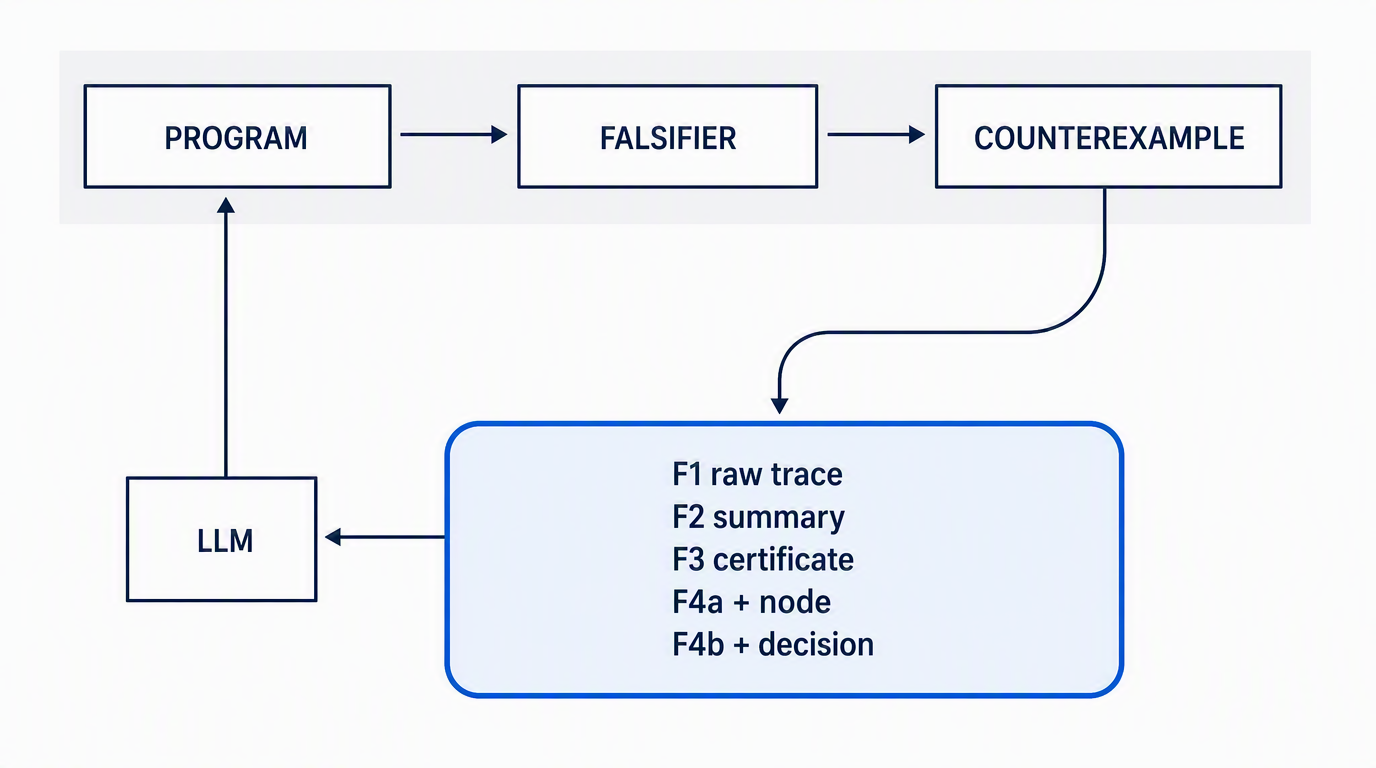
\includegraphics[width=0.92\linewidth]{figures/fig1_pipeline.png}
\caption{The ablation. Falsifier, frozen program, counterexample corpus, token
budget and evaluation suite are identical across all five conditions (grey
band). Only the rendering of the failure into text differs (highlighted). The
corpus is banked once and read by every condition, so minimization and
boundary-search cost are amortized rather than charged to the structured
conditions.}
\label{fig:pipeline}
\end{figure}

\section{Related Work}
\label{sec:related}

\paragraph{LLMs that write control programs.}
Code-as-policies approaches have language models emit executable
policies~\citep{liang2023codeaspolicies}, with prompt construction following the
import-block convention of ProgPrompt~\citep{singh2023progprompt}. These
synthesize but do not falsify.

\paragraph{Adversarial scenario generation.}
Falsification and adversarial scenario search for driving policies are well
established~\citep{wang2021advsim}, with declarative scenario specification
following Scenic~\citep{fremont2019scenic}. These falsify, but where they repair
at all they do so by retraining weights or augmenting data.

\paragraph{Counterexample-guided LLM repair.}
Closest to this work, \citet{orvalho2025cegis} run a CEGIS loop with an LLM
synthesizer over introductory programming assignments, using a test suite as the
oracle and MaxSAT-based fault localization to produce a bug-free program sketch.
They find that counterexample guidance substantially improves repair across six
models and yields smaller fixes. Their question and ours are complementary rather
than competing: they ask whether counterexample feedback helps at all and find
that it does, whereas we hold the counterexample fixed and ask whether adding
formal structure to its rendering helps further. Our null is therefore not in
tension with their positive result. Two differences in setting are worth noting.
Their oracle is a test suite over discrete inputs; ours is a robustness falsifier
over a continuous scenario space, so a counterexample carries a signed margin and
a failing region rather than a single failing input. And their programs are
scored only on correctness, whereas ours must satisfy a safety specification
\emph{and} complete a task, which is precisely the tension \S\ref{sec:dsl}
turns on.

\paragraph{LLM self-repair.}
Self-Refine~\citep{madaan2023selfrefine}, Reflexion~\citep{shinn2023reflexion}
and Self-Debugging~\citep{chen2024selfdebug} iterate on free-form or test-derived
feedback, and two results from that work shaped this design directly.
Reflexion's ablation removes the natural-language self-reflection step and finds
that performance returns exactly to baseline, $0.60$ pass@1 against $0.60$ for
the base model, where full Reflexion reaches $0.68$. Every structured condition
here therefore carries a verbalized narrative alongside its structured fields.
Self-Debugging reports that adding an execution trace to unit-test feedback
\emph{lowers} accuracy on TransCoder, $87.9\%$ against $91.6\%$ for unit-test
feedback alone. More structure is evidently not monotonically better, and we
recorded in advance that we did not assume it would be.

\section{Method}
\label{sec:method}

\subsection{Task, simulator, and contracts}

The task is an unprotected left turn, a permissive circular green rather than a
green arrow, at a fixed signalised four-way junction in
CARLA~\citep{dosovitskiy2017carla} Town05, recorded by exact junction
identifier. The simulator runs synchronously at \mbox{20\,Hz} with fixed physics
substepping. Sensing is ground-truth state and weather is fixed.

\paragraph{Reproducibility, stated precisely.}
The ego trajectory reproduces bit-identically under identical scenario
parameters, both within a process and across process restarts, and four of the
five contracts reproduce exactly. The exception is $\rhoc{4}$, which varies by up
to \mbox{0.69\,m} because the lead vehicle's braking trigger tests a position read
back from the simulator rather than integrating its own state; sub-centimetre
noise there shifts the tick on which deceleration begins. We report this rather
than claiming blanket determinism. $\rhoc{4}$ was the binding contract in $0$ of
$300$ attempts, so no result below depends on it, but it would corrupt any future
result in which it binds.

\begin{table}[t]
\centering
\small
\begin{tabular}{@{}llll@{}}
\toprule
& \textbf{Contract} & \textbf{Robustness} & \textbf{Threshold} \\
\midrule
$\rhoc{1}$ & no collision & metres of bounding-box clearance & $\geq 0$ \\
$\rhoc{2}$ & yield to oncoming & seconds of margin above $\tau_{\text{yield}}$ & 3.0\,s \\
$\rhoc{3}$ & do not enter on red & seconds of green remaining at entry & $\geq 0$ \\
$\rhoc{4}$ & RSS distance to lead & metres above the safe distance & RSS Lemma 2 \\
$\rhoc{5}$ & kinematic comfort & m/s$^2$ of headroom & 3.0\,m/s$^2$ \\
\bottomrule
\end{tabular}
\caption{The five contracts, in signal temporal logic over logged trajectories
using space robustness~\citep{donze2010robust}. Overall robustness is
$\rho = \min_i \rhoc{i}$, so the argmin identifies both the weakest contract and
the timestep at which it is weakest. $\rhoc{4}$ uses the same-direction safe
longitudinal distance of \citet{shalevshwartz2017rss}; $\rhoc{2}$ is that work's
rule~3 and the avoidability filter is its rule~5.}
\label{tab:contracts}
\end{table}

Conjunction as minimum gives blame localization for free, and masks every
contract except the weakest. We therefore report per-contract robustness rather
than $\rho$ alone; \S\ref{sec:regression} gives a result invisible under the
minimum.

\subsection{Program representation and baseline}

The policy is a behaviour tree in a small domain-specific language, parsed to an
AST we own and compiled to \texttt{py\_trees}. Owning the AST is what enables
tree edit distance, node-level blame, and validation before execution.
Composites compile without memory, so every condition is re-evaluated from the
root on each tick.

The baseline is LLM-synthesized from one fixed prompt, sampled 20 times, of which
14 were syntactically valid, then \emph{selected} against two gates measured on a
shared 100-scenario calibration set: a violation rate in $[0.20,0.40]$, and task
completion above $60\%$, the latter because a program can reach a low violation
rate simply by never entering the junction. The frozen baseline violates on
$20.0\%$ of calibration scenarios, enters the junction in $100\%$, and completes
the turn in $88.3\%$. We report the full distribution of all 14 candidates rather
than the selected one alone.

\subsection{Falsification, certificates, and the five conditions}
\label{sec:conditions}

The falsifier samples a six-parameter scenario space uniformly, then refines
locally around low-robustness points, ranking on per-contract robustness rather
than $\rho$ because one parameter moves $\rhoc{1}$ and $\rhoc{2}$ in opposite
directions and the minimum cancels it. Plausibility constraints are enforced at
sample time following Scenic~\citep{fremont2019scenic}. Each admitted
counterexample is minimal (delta-debugged~\citep{zeller2002delta}), generalized
(each surviving parameter binary-searched to where $\rho$ crosses zero),
actionable (a violation-free response existed), and verbalized. We banked
$K{=}20$ counterexamples at a mean cost of $26.6$ simulations each.

\begin{table}[t]
\centering
\small
\begin{tabular}{@{}lll@{}}
\toprule
\textbf{Condition} & \textbf{Feedback block} & \textbf{Prompt tokens (med.)} \\
\midrule
F1 & raw trajectory excerpt around the violation & 16{,}381 \\
F2 & natural-language narrative only & 4{,}584 \\
F3 & contract, $\rho$, per-contract $\rhoc{i}$, minimal params, boundary, narrative & 4{,}780 \\
F4a & F3 plus \texttt{active\_node} & 4{,}871 \\
F4b & F3 plus \texttt{authorising\_node} & 4{,}867 \\
\bottomrule
\end{tabular}
\caption{The manipulated variable. All five share one template with a single
feedback placeholder; we verify mechanically that the 10{,}874 bytes of prefix
and 102 bytes of suffix are byte-identical across all five conditions and all
twenty certificates, splitting by index rather than by string replacement so a
feedback block containing scaffolding text could not disguise a difference.}
\label{tab:conditions}
\end{table}

F1 is not a subset of the other conditions in either direction. The raw trace
carries the behaviour-tree node columns, so it contains the blame signal F2 and
F3 lack, unlabelled and unaggregated but present. At the same time an unwindowed
F1 prompt measures 202{,}812 tokens at the median, $10.1\times$ the per-attempt
budget of 20{,}000, so it must be windowed, and the largest window fitting every
certificate ($\pm 10$ rows) cannot reach the transition F4b names, which lies 28
to 47 rows back in all twenty cases. The ordering is one of structure, not of
information content.

\paragraph{Scope, as planned and as run.}
The pre-registered plan specified three contracts and four scenario parameters.
We ran five and six. The change was made before the baseline was frozen and for a
measured reason: on the reference program under three contracts, the violated
contract determined the blamed leaf exactly, so blame localization carried no
information beyond the contract label and the F3/F4 contrast would have been
vacuous by construction. We re-enabled the red-light and lead-distance contracts
to widen the range of failure modes, and the parameter space grew to six because
two of those parameters are what make the new contracts bind. We report this
because it is a deviation from the plan, and because it did not have the intended
effect: adding contracts does not by itself break the collapse, since each
contract may still map to a single leaf. What addressed it was the alternative
blame definition below, which is exploratory and labelled as such throughout.
The pre-registered field is \texttt{active\_node}; \texttt{authorising\_node} was
defined after observing that the first was constant, and no claim in this paper
rests on F4b outperforming F3.

\paragraph{Generation settings.}
All calls use \texttt{claude-opus-5} at effort \texttt{high}, streaming, with
\texttt{max\_tokens} $=48{,}000$ and prompt caching on the invariant system
block. The model exposes no temperature, \texttt{top\_p} or \texttt{top\_k}
parameter; \texttt{effort} is the only sampling control and is held constant.
The served model identifier is logged per call rather than the requested one.
Consequently the replicate index is not a sampling seed: replicates are
independent samples, not reproducible ones. We measured $3.00$ distinct programs
per (condition, certificate) cell out of $3$.

Two token limits appear in this paper and they constrain different things.
$B = 20{,}000$ is a \emph{prompt} budget, a per-attempt cap on the input we are
willing to spend on rendering a counterexample, and it is what forces F1 to be
windowed. \texttt{max\_tokens} $=48{,}000$ is a \emph{generation} cap on the
model's output for a single call, set high enough that no response was truncated;
across all 300 attempts none hit it. Neither constrains the other, and no attempt
was limited by either.

\section{Results}
\label{sec:results}

Five conditions, twenty certificates and three replicates give 300 repair
attempts. Each patched program is evaluated on 61 scenarios: the counterexample,
a 30-scenario regression suite the baseline passes, and a 30-scenario held-out
suite drawn from a reserved interior region the falsifier never sampled.
Outcomes fall in three buckets never pooled: \emph{truncated} (generation hit the
output cap, a harness failure), \emph{malformed} (validator rejection), and
\emph{ok}. Across all 300 attempts we observed no malformed and no truncated
outputs, so every failure is a valid program that did not fix the problem.

\subsection{Feedback format determines the kind of repair}
\label{sec:patchtype}

Every patch is a hole fill, changing a threshold, or a skeleton edit, inserting,
removing or reordering a node. This is the largest and most robust
condition-dependent effect we measure.

\begin{table}[t]
\centering
\small
\begin{tabular}{@{}lrrrrr@{}}
\toprule
& F1 & F2 & F3 & F4a & F4b \\
\midrule
skeleton edits (of 60) & \textbf{59} & 13 & 15 & 15 & 28 \\
\bottomrule
\end{tabular}
\caption{Structural-edit counts by condition. F1 versus F2 is a $76.7$-point
difference, $95\%$ interval $[+61.7,+90.0]$, from a bootstrap clustered on
certificate.}
\label{tab:patchtype}
\end{table}

\begin{figure}[t]
\centering
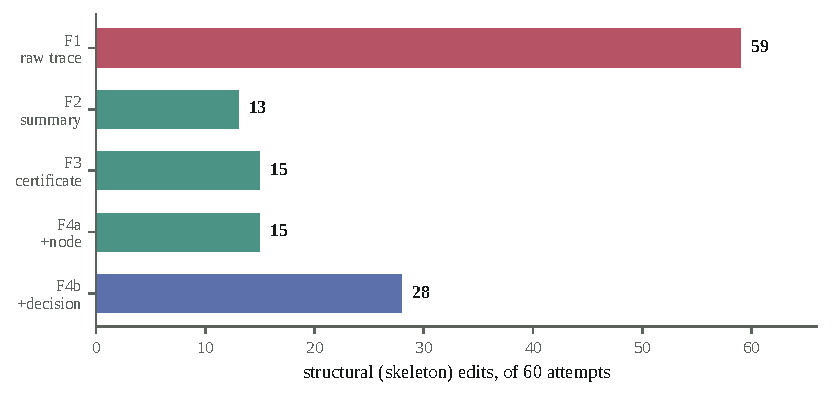
\includegraphics[width=0.80\linewidth]{figures/fig3_patch_type.pdf}
\caption{Structural edits by condition, out of 60 attempts each. Raw trajectory
data drives the model to restructure the program almost every time; a
natural-language summary drives it to adjust a threshold instead.}
\label{fig:patchtype}
\end{figure}

Raw trajectory data drives restructuring in $98.3\%$ of attempts; a
natural-language summary does so in $21.7\%$. F4b sits between the others at
$46.7\%$, and the direction is mechanistically sensible, since naming the
decision that authorised the failing action points at a branch whereas naming a
violated threshold points at a number. We report that as consistent with a
mechanism rather than as a resolved difference: its interval against F3 is
$[-3.3,+45.0]$ and includes zero.

The robust claim is narrower than "more structure gives more control", and we
state it as such. The ordering is not monotone in structure: the least processed
condition produces the most structural edits, and the most processed conditions
produce among the fewest. What is resolvable at this sample size is that the
raw-trace condition is qualitatively different from every processed condition.
For a system designer that is still directly actionable, because the rendering is
a lever on the edit distribution even where it is not a lever on success.

\subsection{Contract satisfaction is trivially achievable by refusing to act}
\label{sec:refusal}

The pre-registered success criterion is $\rho \geq 0$ on the failing scenario
after the patch. A program that never enters the junction satisfies it for free:
$\rhoc{2}$ and $\rhoc{3}$ become vacuous, since one cannot fail to yield without
entering, and are excluded from the argmin; $\rhoc{1}$ is satisfied because no
actor is ever nearby; and $\rho$ falls through to $\rhoc{5}$, which a stationary
vehicle passes comfortably.

\begin{figure}[t]
\centering
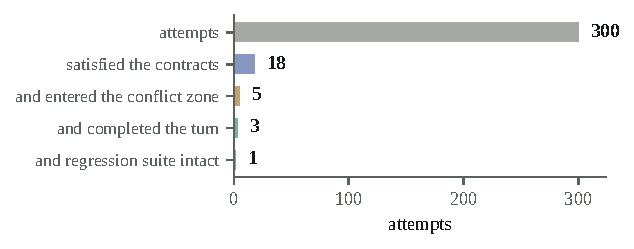
\includegraphics[width=0.80\linewidth]{figures/fig4_funnel.pdf}
\caption{From 300 attempts to one clean repair. The unpatched baseline entered
the junction in 20 of 20 counterexample scenarios, so the paralysis is introduced
by the patches rather than inherited.}
\label{fig:funnel}
\end{figure}

This is the synthesis-side analogue of \emph{vacuous satisfaction} in model
checking, where a specification passes for reasons unrelated to the behaviour it
was written to constrain, and where detecting such passes is a standard
obligation rather than an
afterthought~\citep{beer1997vacuity,kupferman2003vacuity}. Vacuity detection asks
whether a formula held trivially; the analogous question for repair is whether a
patch satisfied the contracts by making them inapplicable, and on this corpus it
usually did.

Thirteen of the eighteen apparent repairs, $72\%$, are of this kind. Three
attempts both satisfied the contract and completed the manoeuvre, and of those
three, only one also left the regression suite intact. Across 300 attempts there
is exactly one clean repair.

The obvious defence is to measure task completion as well, and it does not work
as usually implemented. Our completion metrics were computed over the
60-scenario evaluation suite while success was computed on the single
counterexample scenario. In a pilot run, suite completion read $0.93$ while the
counterexample itself timed out with the vehicle stationary. Nothing was
measuring task completion on the scenario the success metric reads from. Any
evaluation of repaired safety policies that scores specification satisfaction on
one input distribution and task completion on another inherits this defect.

\subsection{Why repair converges on refusal, and what the language permits}
\label{sec:dsl}

With no malformed outputs, every failure is a valid program that did not fix the
problem, which leaves open whether the language could express a correct repair at
all. We tested this constructively, writing candidate repairs by hand in the same
vocabulary and running them on all twenty counterexamples.

\begin{table}[t]
\centering
\small
\begin{tabular}{@{}lrrl@{}}
\toprule
\textbf{Repair} & \textbf{Fixed} & \textbf{Completed} & \textbf{Why} \\
\midrule
frozen baseline & 0/20 & 2/20 & \\
raise gap requirement $5.5 \rightarrow 9.0$ & 0/20 & 3/20 & branch never reached \\
gap guard on committing branch, up to 15.0 & 0/20 & 2/20 & guard passes at every value \\
geometric guard on committing branch & 0/20 & 2/20 & blocks, ego creeps in anyway \\
geometric guard $+$ true stop & 20/20 & 0/20 & never enters the junction \\
\midrule
\textbf{the model's clean repair, from F1} & \textbf{20/20} & \textbf{20/20} & \\
\bottomrule
\end{tabular}
\caption{Constructive test of expressiveness. Each row is a valid program in the
same DSL run on all twenty counterexamples. The final row is the single attempt
of 300 that resolved its counterexample, completed the manoeuvre and caused no
regression, re-evaluated here across the whole corpus.}
\label{tab:dsl}
\end{table}

Three mechanisms make the degenerate answer easy to reach, each measured rather
than inferred. First, the baseline's committing branch is guarded only by a
stop-line distance test satisfied once the ego is \emph{past} the line, and it
outranks the gap-guarded branch, so the gap thresholds are unreachable and
raising them changes nothing. Second, the yield predicate is structurally blind
to a stationary obstacle: it reports time-to-arrival and, to keep the arithmetic
well defined, excludes any vehicle slower than \mbox{0.5\,m/s}, so in one failing
scenario a vehicle \mbox{9.4\,m} away at \mbox{0.04\,m/s} is discarded, the
predicate returns its 30\,s cap, and a guard demanding 15\,s of gap passes while
that car occupies the junction. Third, the geometric predicate does see it and
does block the turn, but the fallback decelerates to \mbox{1.0\,m/s} rather than
to rest, so the ego creeps across the boundary two seconds later and an unguarded
branch commits.

Making the fallback a true stop resolves all twenty counterexamples and completes
none of them. That is the degenerate repair, and it is easy to reach.

\paragraph{A safe and completing repair is nonetheless expressible.}
One attempt in 300, under the raw-trace condition F1, produced a program that
resolved its counterexample, completed the manoeuvre and caused no regression
failure. Re-evaluated across all twenty
counterexamples, including the nineteen it was never shown, \textbf{it resolves
and completes every one}. Its patch adds a geometric guard to the committing
branch and leaves the fallback able to creep, which is sufficient where our
hand-written true stop was over-conservative. Its own comment diagnoses the
mechanism correctly, noting that a stalled vehicle reports an effectively
infinite time-to-conflict-zone so the gap test cannot see it and the path check
must reach far enough to.

So the vocabulary is not the binding constraint. The search is. A safe,
completing, generalising repair exists in this language and was found once in
three hundred attempts, while $72\%$ of apparent repairs converged on the
degenerate answer instead. What the specification rewards determines which of the
two is easier to find, and rewarding only safety makes the degenerate one easier.

We state the limit plainly. Our hand-written repairs were a family of natural
single- and double-edit candidates, not an exhaustive search, so \emph{none of
the hand-written repairs tested achieved both across all twenty counterexamples};
we do not claim no such repair exists, and indeed the model found one.

\paragraph{Validation.} Because one contract is known to vary by up to
\mbox{0.69\,m} over identical parameters (\S\ref{sec:method}), we repeated the
clean repair's evaluation on its own counterexample six times. Robustness
reproduced exactly, with zero spread in $\rho$ and zero spread in $\rhoc{4}$, and
$\rhoc{4}$ was never the binding contract. The verdict does not depend on that
variability.

\subsection{Repair success: no detected improvement}
\label{sec:null}

\begin{figure}[t]
\centering
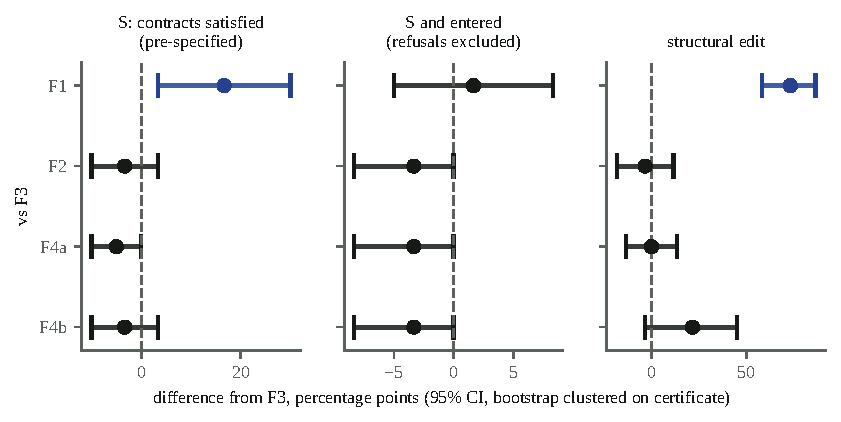
\includegraphics[width=\linewidth]{figures/fig2_uncertainty.pdf}
\caption{Paired differences against F3 with $95\%$ intervals from a bootstrap
clustered on certificate, which respects both the shared counterexample corpus
and the three repeated attempts per cell. Only the raw-trace condition separates
from zero, and on repair success that separation is an artifact of
resolution-by-refusal: excluding refusals it falls inside the interval with
everything else.}
\label{fig:uncertainty}
\end{figure}

\begin{table}[t]
\centering
\small
\begin{tabular}{@{}lrrrrr@{}}
\toprule
\textbf{Cond.} & \textbf{Fix rate} & \textbf{Ex-refusal} & \textbf{Fixed \& drove} & \textbf{Broke $\geq 1$} & \textbf{Mean TED} \\
\midrule
F1  & 21.7\% & 5.0\% & 1/60 & 42/60 & 5.93 \\
F2  &  1.7\% & 0.0\% & 0/60 & 37/60 & 5.77 \\
F3  &  5.0\% & 3.3\% & 2/60 & 44/60 & 6.95 \\
F4a &  0.0\% & 0.0\% & 0/60 & 54/60 & 7.38 \\
F4b &  1.7\% & 0.0\% & 0/60 & 47/60 & 4.27 \\
\bottomrule
\end{tabular}
\caption{Repair success over 300 attempts. Every paired difference against F3
has a $95\%$ interval containing zero once refusals are excluded.}
\label{tab:main}
\end{table}

After excluding refusals we did not detect a reliable improvement in repair
success from any feedback format. Every paired comparison against F3 has an
interval containing zero. We note that an interval containing zero is not
evidence that the effect is absent, only that this design did not resolve one. The raw-trace condition clears zero on the
pre-registered rate, but ten of its thirteen resolutions are refusals, and
excluding those the difference is $+1.7$ with an interval of $[-5.0,+8.3]$.

We make no significance claim, and we do not claim a null. With $K{=}20$
counterexamples, three replicates and between zero and thirteen successes per
condition, the design supports neither.

\subsection{Repair is net destructive, and the minimum hides part of it}
\label{sec:regression}

Across all 300 attempts, 224 ($74.7\%$) caused at least one previously-passing
regression scenario to fail, against 18 apparent fixes. The modal outcome of a
repair attempt is that it did not fix the counterexample and broke one thing that
worked. This holds in every condition.

Per-contract reporting reveals a second effect invisible under the minimum:
$\rhoc{5}$ degrades in every condition without exception, from $1.000$ to between
$0.59$ and $0.93$. Every feedback format pushes the model toward harder braking
and faster commits, and whenever $\rhoc{1}$ is the argmin this is masked
completely. Generalization changes span $+0.021$ to $+0.039$, a $1.8$-point
spread well inside the intervals of \S\ref{sec:null}.

\subsection{When blame localization can carry information}
\label{sec:blame}

Resolving blame to the leaf executing at the argmin is vacuous for any program
whose commit branch is guarded by a region test, whenever the violated contracts
are evaluated over that same region, because the guard leaves exactly one leaf
reachable there. On our baseline $H(\texttt{active\_node} \mid \text{contract}) =
0.000$ bits against $H(\text{contract}) = 1.234$ bits. This is a property of
program structure and not of contract count: we verified by construction that
five contracts each blaming one node still yields $\Hnc = 0$.

We therefore propose a precondition, cheap to check before running any such
experiment:
\[
  \Hnc > 0 .
\]
Where it fails, the blame field is a deterministic re-encoding of the contract
label and carries no information beyond it. We stop short of calling such a
condition a placebo: redundant text can still influence a language model's
output, which is precisely why we do not treat F4a as a measure of the
experiment's resolution. Defining blame instead as the
last distinct leaf active before the failing leaf began running, which is the
decision that authorised the action rather than the action executing when the
consequence landed, raises this to $0.500$ bits on the same corpus. We report
both, note that the second was defined after observing the first was vacuous, and
make no claim that F4b outperforms F3.

\section{Limitations}
\label{sec:limitations}

Two limitations deserve more than a clause. First, \textbf{every result is
conditioned on a single frozen baseline program}. The structural argument of
\S\ref{sec:blame} generalises, since it depends only on a commit branch guarded by
a region test, but no effect size here is claimed to transfer to another program.
A second baseline would test that directly and is the most valuable single
extension we can identify; it would also tell us whether the refusal attractor of
\S\ref{sec:dsl} is a property of this program's branch ordering or of the task.
Second, \textbf{the expressiveness audit is not exhaustive}. We wrote a family of
natural single- and double-edit repairs and ran them; we did not search the
program space. That family failed to find a safe and completing repair, and the
model found one, which is direct evidence that the family was incomplete rather
than that the language was. Any statement here about what the DSL permits should
be read as a statement about what these candidates reached.

The remaining limitations are ordinary. $K{=}20$ with three replicates supports no
significance claim, and an interval containing zero is not evidence of absence. We
measure one repair step per counterexample rather than compounding effects over
rounds. F1 is not a subset of the other conditions in either direction
(\S\ref{sec:conditions}), so the ordering is one of structure rather than
information content. F1 also differs in \emph{length} as well as in kind, at
roughly 16{,}400 prompt tokens against about 4{,}700 for every other
condition, so the edit-type contrast of \S\ref{sec:patchtype} cannot separate
the effect of raw signal from the effect of prompt volume. Seven of twenty certificates report no boundary, because
their sole boundary parameter was measured to be anti-correlated with the quantity
it names and was suppressed; those degrade to point counterexamples. Corpus
construction is amortized across all five conditions, so the cost asymmetry a
deployed closed loop would face is absent here. The simulator reproduces
bit-identically but the model does not, since it exposes no seed or temperature.
Oncoming vehicles travel at constant velocity, making the scenario harsher than
naturalistic traffic.

\section{Conclusion}

Formal structure in counterexample feedback changes what repair is attempted,
substantially and robustly, with raw execution traces driving structural rewrites
where processed feedback drives threshold adjustments. After excluding refusals we
did not detect a reliable improvement in repair success from any feedback format,
which at this sample size is a statement about our resolution rather than about
the effect.

The more useful finding came from asking why so many apparent repairs stopped
driving. Contract satisfaction on a failing scenario is trivially achievable by
inaction, and the usual defence of also measuring completion fails when
completion is scored on a different input distribution. A safe and completing
program does exist in this language, and one attempt in three hundred found it
and generalised to the whole corpus. Repair converged on refusal not because the
vocabulary forbade the alternative but because the specification made the
degenerate answer easier to find.

We suggest this generalises. Where a repair task scores only specification
satisfaction, and the program representation admits inaction, counterexample-guided
repair should be expected to converge on inaction, and the fix belongs in the
task specification rather than in the feedback.

\bibliographystyle{plainnat}
\bibliography{references}

\end{document}
